\documentclass[conference]{IEEEtran}
\usepackage{graphicx}


% path gambar
\graphicspath{{./picture/}}

% JUDUL %%%%%%%%%%%%%%%%%%%%%%%%%%%%%%%%%%%%%%%%%%%%%%%%%%%%%
\title{Mengirim Data Signal Strength Hasil Pemindaian Jaringan WiFi menggunakan NodeMCU V3 ke Telegram Dengan Channel BotFather}

% PENULIS %%%%%%%%%%%%%%%%%%%%%%%%%%%%%%%%%%%%%%%%%%%%%%%%%%%
\author{Johanes Wilian Ang\IEEEauthorrefmark{1},Erwin Erikson\IEEEauthorrefmark{2},Johnny\IEEEauthorrefmark{3}, Andrian Syah\IEEEauthorrefmark{4}\\
\textit{Fakultas Teknologi Informasi}\\
\textit{Teknik Komputer}\\
\textit{Institut Teknologi Batam}\\
Batam, Indonesia\\
Email: \{\IEEEauthorrefmark{1}1822002,\IEEEauthorrefmark{2}1822003,\IEEEauthorrefmark{3}1822004,\IEEEauthorrefmark{4}1922009\}@student.iteba.ac.id}

\begin{document}
% untuk mengeluarkan judul dan author
\maketitle
% ABSTRAK %%%%%%%%%%%%%%%%%%%%%%%%%%%%%%%%%%%%%%%%%%%%%%%%%%
\begin{abstract}
    Dalam sistem komunikasi data berbasis \emph{wireless}, pemanfaatan \emph{WiFi} 
    menjadi pilihan banyak pengguna karena keunggulan mobilitas dan kecepatan transfer data.
    Kualitas \emph{signal strength} sangat berpengaruh dalam layanan komunikasi data ini, 
    sehingga kualitas \emph{signal strength} pada jaringan \emph{WiFi} perlu diketahui.
    Pemindaian jaringan \emph{WiFi} menggunakan perangkat \emph{NodeMCU V3} dapat mengukur \emph{signal strength} dari 
    masing-masing jaringan, lalu data hasil pemindaian dan pengukuran \emph{signal strength} dikirim ke
    Telegram menggunakan \emph{channel} BotFather melalui \emph{webserver} agar dapat diketahui hasilnya.
\end{abstract}
\vspace{0.2cm}
% kata kunci %%%%%%%%%%%%%%%%%%%%%%%%%%%%%%%%%%%%%%%%%%%%%%%%
\begin{IEEEkeywords}
    \emph{WiFi}, \emph{signal strength}, \emph{NodeMCU V3}, \emph{webserver}, \emph{BotFather}
\end{IEEEkeywords}
% pendahuluan %%%%%%%%%%%%%%%%%%%%%%%%%%%%%%%%%%%%%%%%%%%%%%
\section{Pendahuluan}
Perkembangan teknologi merupakan hal yang sejalan dengan 
perkembangan zaman, dimana masyarakat kini selalu
menginginkan berbagai hal agar dapat dilakukan secara otomatis
ataupun dari jarak jauh. Perkembangan smarthome dengan
kontrol jarak jauh menjadi salah satu fokus utama dalam
perkembangan teknologi dimana pengontrolannya dilakukan dari
jarak jauh dan secara real time dan diharapkan pula bagi generasi
masa kini untuk dapat mengimplementasikan beberapa bagian
dari teknologi yang cukup sederhana dalam lingkungan masyarakat. ada
beberapa teknik analisis yang di gunakan untuk menentukan
sistem, perangkat dan juga bagaimana pengaplikasiannya. Maka
dari itu dipilihlah Telegram bot sebagai interface antara perangkat
dan pengguna dimana board ESP8266 Module sebagai pusat
kontrolnya dan pemrogramannya menggunakan Ardiono IDE.
Semua hal ini masih perlu di pelajari terlebih dahulu dengan
dukungan berbagai jurnal penelitian ,
    
    Setelah proses analisis dilakukan maka akan didapat hasil
berupa suatu sistem notifikasi scanner yang di program untuk dapat
dikontrol dari jarak jauh. Pengontrolan ini dilakukan dengan
bantuan internet sebagai media penghubungnya dan juga Bot
Telegram sebagai media penginputan perintah yang diberikan
dengan jarak yang jauh apabila terdapat koneksi internet 
antara perangkat penerima dan juga pengirim 


\section{Penjelasan}
\subsection{Bot Telegram}
\vspace{0.2cm}
\begin{figure}[h]
    \centering
    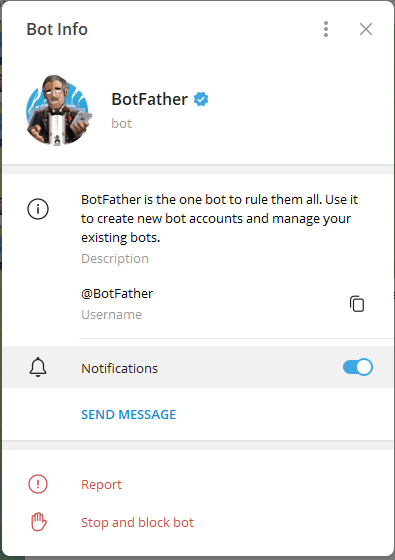
\includegraphics[width=0.2\textwidth]{Botfather.png}
    \caption{BotFather Telegram}
\end{figure}

    Telegram adalah salah satu platform perpesanan sejenis dengan
    WhatApps, dimana sistem perpesanan di telegram juga bisa mencakup
    lintas platform. Bot Telegram 
    sendiri merupakan salah satu fitur dari Telegram yang mana funginya untuk
    mempermudah kegiatan dalam mengakses Telegram. Bot itu sendiri
    berasal dari kata robot atau mesin pekerja yang meringkankan pekerjaan.
    Bot di dalam telegram bekerja dengan cara inputan perintah yang buat.
    Dalam pengaturan atau pebuatan bot telegram ada dua cara yang 
    bisa dilakukan, yang pertama dengan membuat program dengan bahasa
    mesin lalu diinput ke protokol telegram. dan yang kedua yaitu dengan
    meminta akses bot telegram ke BotFather.
   
    
        Membuat bot Telegram dengan meminta Akses kepada BotFather dilakukan untuk
    mendapatkan kode API, kode ini merupakan kode unik khusus bagi suatu
    akun Bot Telegram untuk Koneksi dengan sistem di luar Telegram itu
    sendiri. Cara kerja kode ini mirip seperti nomor HP, yang mana setiap
    penguna Bot Telegram memiliki kode API tersendiri dan tidak dapat di copy
    oleh orang lain, namun jika pengguna ingin mengubah kode API yang
    dimilikinya bisa dilakukan dengan cara menghapus Bot Telegram lalu
    membuat ulang Bot Telegram dengan IDE yang sama.
    BotFather sendiri merupakan suatu Fitur AI milik Telegram yang
    mengatur pembuatan Bot Telegram yang bekerja otomatis, sistem
    BotFather ini lebih merujuk ke sistem pembalasan pesan otomatis yang
    mana pemeberian kode API yang diberikan dilakukan secara acak.

    \subsection{NodeMCU}
    NodeMCU versi 0.9 diluncurkan pada 13 Oktober 2014 oleh user bernama Hong pada GitHub setahun setelah diproduksinya ESP8266 pada 30 Desember 2013. ESP8266 merupakan SoC yang memiliki module wifi sebagai perangkat tambahan mikrokontroller agar dapat terhubung dengan wifi dan membuat koneksi TCP/IP.

    NodeMCU merupakan sebuah platform IoT yang bersifat open source dan juga include dengan module ESP 12, dan berjalan pada firmware esp8266 yang menjadikan NodeMCU sebuah mikrokontroller yang telah dilengkapi dengan module Wifi didalamnya.

    \begin{figure}[h]
        \centering
        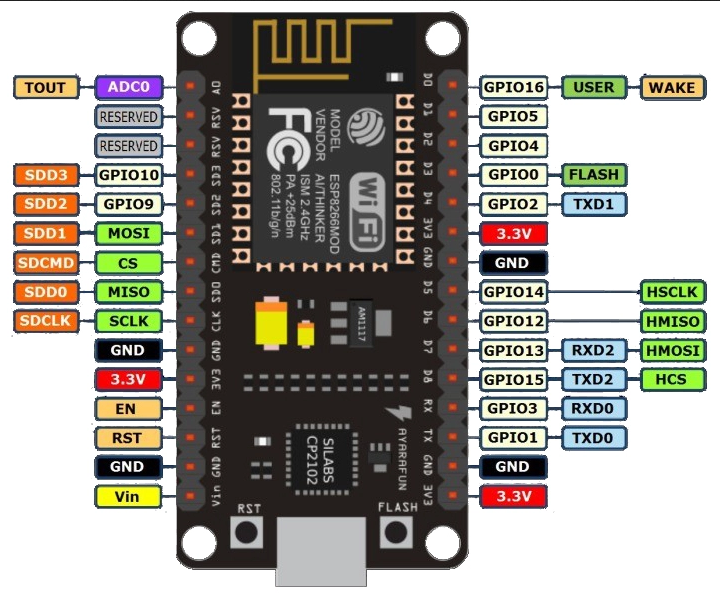
\includegraphics[width=0.3\textwidth]{Nodem.png}
        \caption{GPIO NodeMCU v2}
    \end{figure}

    NodeMCU berfungsi sama seperti Arduino, walaupun dengan IC, GPIO, dan Bahasa program yang digunakan berbeda tetapi tujuannya sama yaitu untuk mengontrol suatu system, dan kelebihannya dibandingkan arduino yaitu telah include dengan module Wifi yang tertanam pada systemnya.

    \subsection{Cloud Hosting}
    \begin{figure}[h]
        \centering
        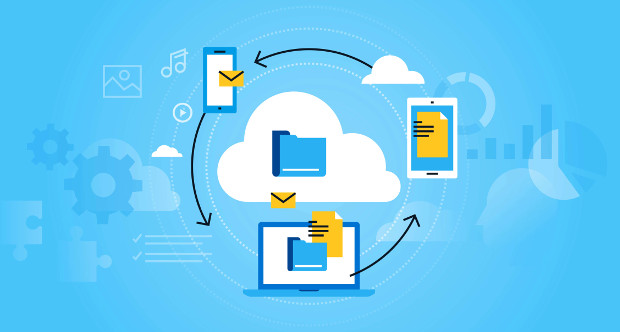
\includegraphics[width=0.4\textwidth]{cloudhosting.jpg}
        \caption{BotFather Telegram}
    \end{figure}

    Cloud hosting adalah jenis hosting yang menggunakan beberapa server untuk menyeimbangkan beban (load) server dan memaksimalkan server uptime.
    Teknologi cloud hosting menggabungkan beberapa server yang bekerja seperti satu server utuh. Gabungan dari beberapa server ini biasanya disebut dengan “cloud cluster”.
    Semakin banyak server yang tergabung di dalam cluster, semakin besar juga resources yang bisa dibagikan oleh cluster tersebut. 
    Jadi saat satu server sedang bermasalah, teknologi ini akan memberikan sumber daya dari server lainnya untuk menjaga agar website Anda bisa tetap berjalan dengan normal.
    Oleh karena itu, cloud hosting dikenal sebagai web hosting yang memiliki reliabilitas dan fleksibilitas yang tinggi dibandingkan dengan jenis web host lainnya.
    Saat ini sudah banyak web owner yang mulai memindahkan situs mereka ke platform cloud. Namun, perlu diingat bahwa solusi hosting ini tidak diperuntukan untuk semua jenis website.
    Misalnya, jika saat ini Anda mengelola situs web dengan lalu lintas rendah dan tidak membutuhkan banyak resources, meningkatkan paket ke cloud hosting mungkin tidak perlu.
    Jika situs web Anda mendapatkan lonjakan lalu lintas yang besar, maka mungkin ingin mempertimbangkan upgrade cloud hosting untuk mencegah server overload.
    \vspace{0.2cm}
    \subsubsection{Kelebihan Cloud Hosting}
      \begin{itemize}
        \item Uptime Lebih Stabil
        \item Scalability
        \item Loading Time Lebih Cepat
        \item Biaya Fleksibel
        \item Data Recovery Lebih Mudah
      \end{itemize}
      \vspace{0.2cm}
      \subsubsection{Kekurangan Cloud Hosting}
      \begin{itemize}
        \item Lebih rentan terkena cyber-attack
        \item Kecepatan server bergantung pada kecepatan internet
        \item Pakai cloud bisa menjadi mahal
      \end{itemize}
    


\section{Hasil dan Pembahasan}
\subsection{Hasil Pengukuran}
Berikut ini perhitungan menggunakan persamaan RSSI 
pada jaringan wireless yang ada disekitar 
kampus iteba terhadap pengahalang



\begin{table}[htbp]
    \caption{Table Analisis Pengukuran RSSI}
    \begin{center}
    \begin{tabular}{|c|c|c|c|}
        \hline
    \textbf{SSID} & \textbf{\textit{Jarak}}& \textbf{\textit{RSSI}}& \textbf{\textit{Penerima Sinyal}} \\
    \hline
    Angeli & 4 meter& -76 dBm & 48  \\
    \hline
    VEGAZUS & 12 meter& -88 dBm & 24  \\
    \hline
    Aldikadek & 2 meter& -36 dBm & 100   \\
    \hline
    \multicolumn{4}{l}{$^{\mathrm{a}}$Hasil dari Integrasi Dari Nodemcu Ke telegram}
    \end{tabular}
    \label{tab1}
    \end{center}
    \end{table}

\subsection{Pengaruh Besar nya Kekuatan sinyal}
Kekuatan sinyal RSSI yang diterima oleh
receiver tidak hanya bergantung pada jarak
antara transmitter dan receiver, akan tetapi
menunjukkan variasi yang besar terhadap fading
dan shadowing pada sebuah lokasi. Hal ini
terlihat pada tempat penelitian yang kondisi
lingkungannya memiliki banyak property seperti
didalam ruangan terdapat sekat, lemari, meja dan
property lainnya, sehingga akan terjadi peredaman sinyal, pembelokan sinyal dan pemantulan
sinyal yang mengakibatkan penurunan kuat
sinyal yang dipancarkan oleh transmiter kepada
receiver, walaupun jarak antara transmiter dan
receiver cukup dekat, namun terhalang oleh
adanya property disekitarnya, maka kekuatan
sinyalnya akan menurun dan kemungkinan
kekuatan sinyal nya akan sama dengan kekuatan
sinyal pada jarak antara transmiter dan receiver
yang cukup jauh, namun tidak memiliki
penghalang disekitarnya.

\section{Kesimpulan}

% referensi %%%%%%%%%%%%%%%%%%%%%%%%%%%%%%%%%%%%%%%%%%%%%%%%
% \bibliographystyle{IEEEtran}
% \bibliography{reference}

\end{document}
